\noindent

\includegraphics[height=1.25cm]{images/pictograms/benchmark}

\includegraphics[height=1.25cm]{images/pictograms/under_construction}

\includegraphics[height=1.25cm]{images/pictograms/FEM}

\includegraphics[height=1.25cm]{images/pictograms/paraview}


%%%%%%%%%%%%%%%%%%%%%%%%%%%%%%%%%%%%%%%%%%%%%%%%%%%%%%%%%%%%%%%%%%%%%%%%%%%%%%%%%%%%%%%%%%%%%%%%%%%

\begin{flushright} {\tiny {\color{gray} python\_codes/fieldstone\_152/text.tex}} \end{flushright}

\lstinputlisting[language=bash,basicstyle=\small]{python_codes/fieldstone_152/keywords.key}

\par\noindent\rule{\textwidth}{0.4pt}

\begin{center}
\inpython
{\small Code: \url{https://github.com/cedrict/fieldstone/tree/master/python_codes/fieldstone_152}}
\end{center}

\par\noindent\rule{\textwidth}{0.4pt}

%{\sl This stone was developed in collaboration with Donald Duck}. \index{contributors}{D. Duck}

%\par\noindent\rule{\textwidth}{0.4pt}

%%%%%%%%%%%%%%%%%%%%%%%%%%%%%%%%%%%%%%%%%%%%%%%%%%%%%%%%%%%%%%%%%%%%%%%%%%%%%%%%%%%%%%%%%%%%%%%%%%%

The code for this \stone is based on \stone~\ref{f21}. 

The goal here is to explore the influence of the mapping polynomial order and/or
the number of quadrature points on the accuracy of the solution of the so-called 
annulus benchmark \ref{MMM-xxxx}.

We will explore:
\begin{itemize}
\item resolution
\item nqperdim=2,3,4,5
\item mapping=Q1,Q2,Q3,Q4
\end{itemize}
and will monitor the computed area, and the velocity and pressure errors.

%%%%%%%%%%%%%%%%%%%%%%%%%%%%%%%
\section*{Areas and volumes}

\begin{center}
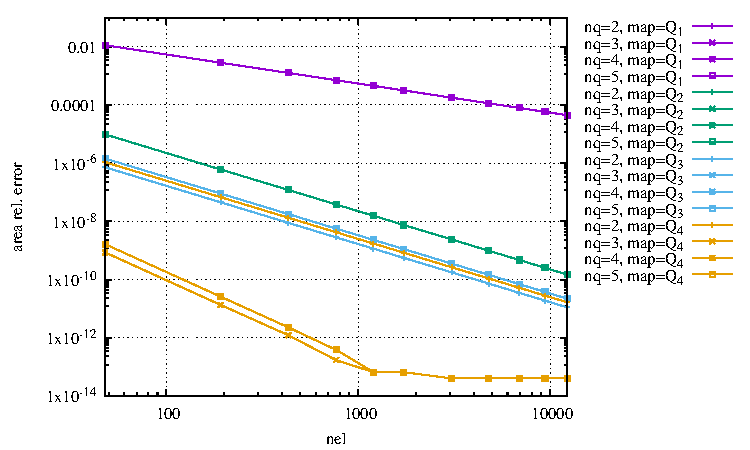
\includegraphics[width=8cm]{python_codes/fieldstone_152/results/areas/areas.pdf}
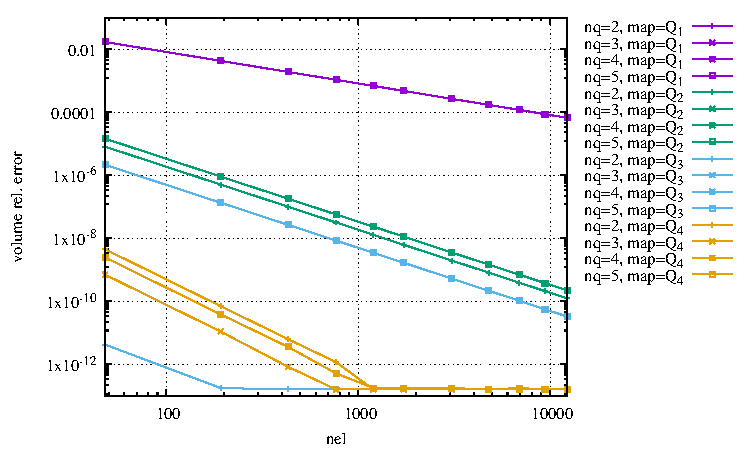
\includegraphics[width=8cm]{python_codes/fieldstone_152/results/areas/volumes.pdf}
\end{center}

Conclusions:
\begin{itemize}
\item unsurprisingly Q1 mapping yields the worst results
\item the type of mapping is the controling factor
\item for the isoparametric mapping $Q_2$ the number of quadrature points 
is not critical. Results are virtually identical for nqperdim=2,3,4,5
\item Q3 about one order of magnitude more accurate than Q2 
\item Q4 mapping 3-4 orders of magnitude more accurate than Q2 mapping
\end{itemize}







%%%%%%%%%%%%%%%%%%%%%%%%%%%%%%%%%%%%%%%%%%%%%%%%%%%%%%%%%%%%%%%%%%%%%%%%%%%%%%%%%%%%%%%%%%%%%%%%%%%
\par\noindent\rule{\textwidth}{0.4pt}

\vspace{.5cm}

\begin{center}
\fbox{\begin{minipage}{0.9\textwidth}
{\color{teal}To Do, open questions, future work?}
\begin{itemize}
\item do smthg
\end{itemize}
\end{minipage}}
\end{center}

%%%%%%%%%%%%%%%%%%%%%%%%%%%%%%%%%%%%%%%%%%%%%%%%%%%%%%%%%%%%%%%%%%%%%%%%%%%%%%%%%%%%%%%%%%%%%%%%%%%
\vspace{.5cm}

\Literature:\\
\fullcite{xxxxYY}


